\documentclass[12pt]{article}
\usepackage[margin=1in]{geometry}
\usepackage{booktabs}
\usepackage{hyperref}
\usepackage{graphicx}
\usepackage{setspace}

\onehalfspacing

\title{\textbf{Problem Set 5}}
\author{Sumedha Ray}
\date{March 10, 2026}

\begin{document}
\maketitle

%% -------------------------------------------------------
\section{Web Scraping: Indian States Literacy Rates (Wikipedia)}
%% -------------------------------------------------------

\subsection*{Data Description}

I scraped the Wikipedia page \textit{List of Indian states and union territories by
literacy rate} (\url{https://en.wikipedia.org/wiki/List_of_Indian_states_and_union_territories_by_literacy_rate})
using the \texttt{rvest} package in R. This page does not provide an API; I parsed
its HTML tables directly. The relevant table contains state- and union-territory-level
total literacy rates across six decennial censuses: 1951, 1961, 1971, 1981, 1991,
2001, and 2011. The resulting dataset has 36 rows (35 states/UTs plus an all-India
total) and 8 columns, and was saved as \texttt{india\_literacy.csv}.

\subsection*{Why This Data Interests Me}

My research looks at the long-run effects of the 2002 Gujarat riots on women's
empowerment using four rounds of the National Family Health Survey (NFHS). Literacy
is one of the key dimensions of women's empowerment I study, and state-level literacy
trends provide important macroeconomic context for my micro-level estimates. Gujarat
in particular shows an interesting trajectory (rising steadily from roughly 22\% in
1951 to 78\% by 2011) which helps situate my within-state analysis.

More broadly, this dataset would be useful for any cross-state analysis of development
outcomes in India. I think, the scraping workflow I developed here could also be extended
to collect other Wikipedia tables on Indian states, such as GDP per capita, sex ratio,
or female labor force participation.

\subsection*{Packages and Resources Used}

I used the \texttt{rvest} package to read and parse the HTML, and \texttt{dplyr} for cleaning. The table was identified by looping over all \texttt{html\_table()} results and inspecting each one. I consulted the \href{https://rvest.tidyverse.org/articles/rvest.html}{\texttt{rvest} vignette} for guidance on \texttt{html\_nodes()} and \texttt{html\_table()} syntax.


%% -------------------------------------------------------
\section{API Data: World Bank Indicators for India}
%% -------------------------------------------------------

\subsection*{Data Description}

I used the \texttt{wbstats} package to look at the World Bank's public API for four development indicators for India, covering 1990 to 2023:

\begin{itemize}
  \item Women owning a bank account (\% of female population), from the Global Findex survey
  \item Intentional homicide rate (per 100,000 people)
  \item Total fertility rate (births per woman)
  \item Maternal mortality ratio (per 100,000 live births)
\end{itemize}

The resulting dataset contains one row per year and I saved it as \texttt{india\_wb\_indicators.csv}.

\subsection*{What I Found}

Figure \ref{fig:bank} shows the trend in women's bank account ownership over time,
and Figure \ref{fig:homicide} shows the intentional homicide rate.Fertility rates have fallen steadily, from roughly 4.0 births per woman in 1990 to around 2.0 by 2020, approaching replacement level. Maternal mortality has similarly
declined, from over 500 per 100,000 live births in 1990 to under 100 by
2020, reflecting improvements in healthcare access.

The bank account ownership data (available only from 2011 onward via the World Bank's
Global Findex survey) shows a sharp rise in financial inclusion among Indian women. The homicide rate data is sparse for India in the World Bank database.

\subsection*{Packages Used}

I used \texttt{wbstats} to interface with the World Bank API, \texttt{dplyr} for
cleaning, and \texttt{ggplot2} for visualization, following plotting conventions
from course notes (e.g., \texttt{theme\_minimal()}, axis label rotation, and
observation count captions).

\section{Figures}

\begin{figure}[h!]
  \centering
  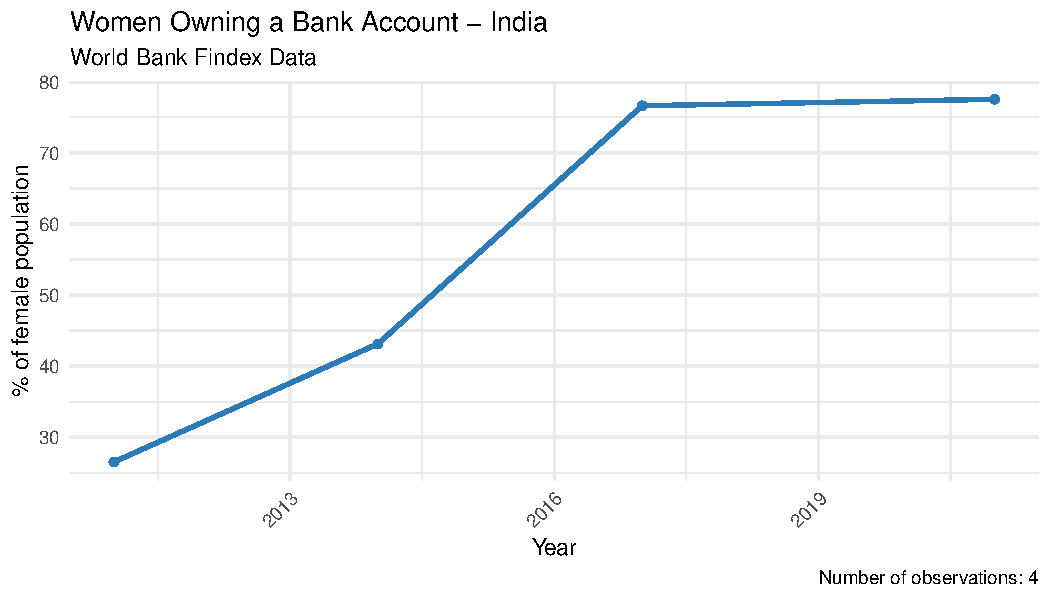
\includegraphics[width=0.6\textwidth]{india_bank_account.pdf}
  \caption{Women Owning a Bank Account, India (World Bank Findex)}
  \label{fig:bank}
\end{figure}

\begin{figure}[h!]
  \centering
  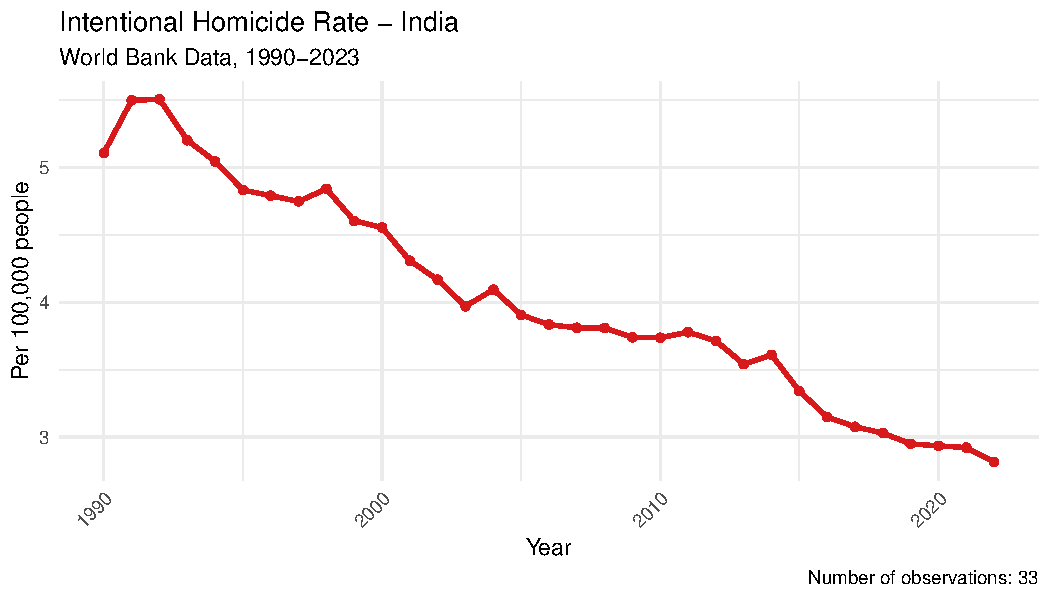
\includegraphics[width=0.6\textwidth]{india_homicide.pdf}
  \caption{Intentional Homicide Rate, India (World Bank)}
  \label{fig:homicide}
\end{figure}

\end{document}